%%%%%%%%%%%%%%%%%%%%%%%%%%%%%%%%%%%%%%%%%%%%%%%%%%%%%%%%%%%%%%%%%%%%%%%%
%    INSTITUTE OF PHYSICS PUBLISHING                                   %
%                                                                      %
%   `Preparing an article for publication in an Institute of Physics   %
%    Publishing journal using LaTeX'                                   %
%                                                                      %
%    LaTeX source code `ioplau2e.tex' used to generate `author         %
%    guidelines', the documentation explaining and demonstrating use   %
%    of the Institute of Physics Publishing LaTeX preprint files       %
%    `iopart.cls, iopart12.clo and iopart10.clo'.                      %
%                                                                      %
%    `ioplau2e.tex' itself uses LaTeX with `iopart.cls'                %
%                                                                      %
%%%%%%%%%%%%%%%%%%%%%%%%%%%%%%%%%%
%
%
% First we have a character check
%
% ! exclamation mark    " double quote  
% # hash                ` opening quote (grave)
% & ampersand           ' closing quote (acute)
% $ dollar              % percent       
% ( open parenthesis    ) close paren.  
% - hyphen              = equals sign
% | vertical bar        ~ tilde         
% @ at sign             _ underscore
% { open curly brace    } close curly   
% [ open square         ] close square bracket
% + plus sign           ; semi-colon    
% * asterisk            : colon
% < open angle bracket  > close angle   
% , comma               . full stop
% ? question mark       / forward slash 
% \ backslash           ^ circumflex
%
% ABCDEFGHIJKLMNOPQRSTUVWXYZ 
% abcdefghijklmnopqrstuvwxyz 
% 1234567890
%
%%%%%%%%%%%%%%%%%%%%%%%%%%%%%%%%%%%%%%%%%%%%%%%%%%%%%%%%%%%%%%%%%%%
%
\documentclass[12pt,a4paper,final]{iopart}
\usepackage[letterpaper]{geometry}
\newcommand{\gguide}{{\it Preparing graphics for IOP journals}}
%Uncomment next line if AMS fonts required
\usepackage{iopams}  
\usepackage{graphicx}
\usepackage[breaklinks=true,colorlinks=true,linkcolor=blue,urlcolor=blue,citecolor=blue]{hyperref}
%\usepackage[T1]{fontenc}
%\usepackage{alltt}
%\usepackage{underscore}

%% Choose Font %%
%\usepackage{fontspec}
%\setmainfont{Fontin}
\usepackage{libertine}
\usepackage{graphicx}

\usepackage[colorlinks=true]{hyperref}

\begin{document}

\title[Information for DOE Report]{Information for DOE Report}
	
\author[cor1]{Shih-Kai Lin}
\address{Colorado State University}
\ead{\mailto{Shihkai.Lin@colostate.edu}}


%\begin{abstract}
%This document describes the  preparation of an article using \LaTeXe\ and 
%\verb"iopart.cls" (the IOP \LaTeXe\ preprint class file).
%This class file is designed to help 
%authors produce preprints in a form suitable for submission to any of the
%journals published by IOP Publishing.
%Authors submitting to any IOP journal, i.e.\ 
%both single- and double-column ones, should follow the guidelines set out here. 
%On acceptance, their TeX code will be converted to 
%the appropriate format for the journal concerned.
%
%\end{abstract}

%Uncomment for PACS numbers title message
%\pacs{00.00, 20.00, 42.10}
% Keywords required only for MST, PB, PMB, PM, JOA, JOB? 
%\vspace{2pc}
%\noindent{\it Keywords}: Article preparation, IOP journals
% Uncomment for Submitted to journal title message
%\submitto{\JPA}
% Comment out if separate title page not required
%\maketitle

\vspace{\baselineskip}
This document summarizes the work I have done in the past year for the DOE report, starting with DUNE and followed by NO$\nu$A.

\section{DUNE}

\subsection{Comparison of Photon Detector Designs at CDDF}
We compared the performance of the photon detector designs from CSU and LSU. Detectors were put side by side in the Dewar at CDDF. Each detector has 2 SiPM channels. Figure~\ref{fig:cddfadc} shows the integrated ADC for the four SiPM channels. A threshold scan was done to set the threshold just above the pedestal peak.

\begin{figure}
  \centering
  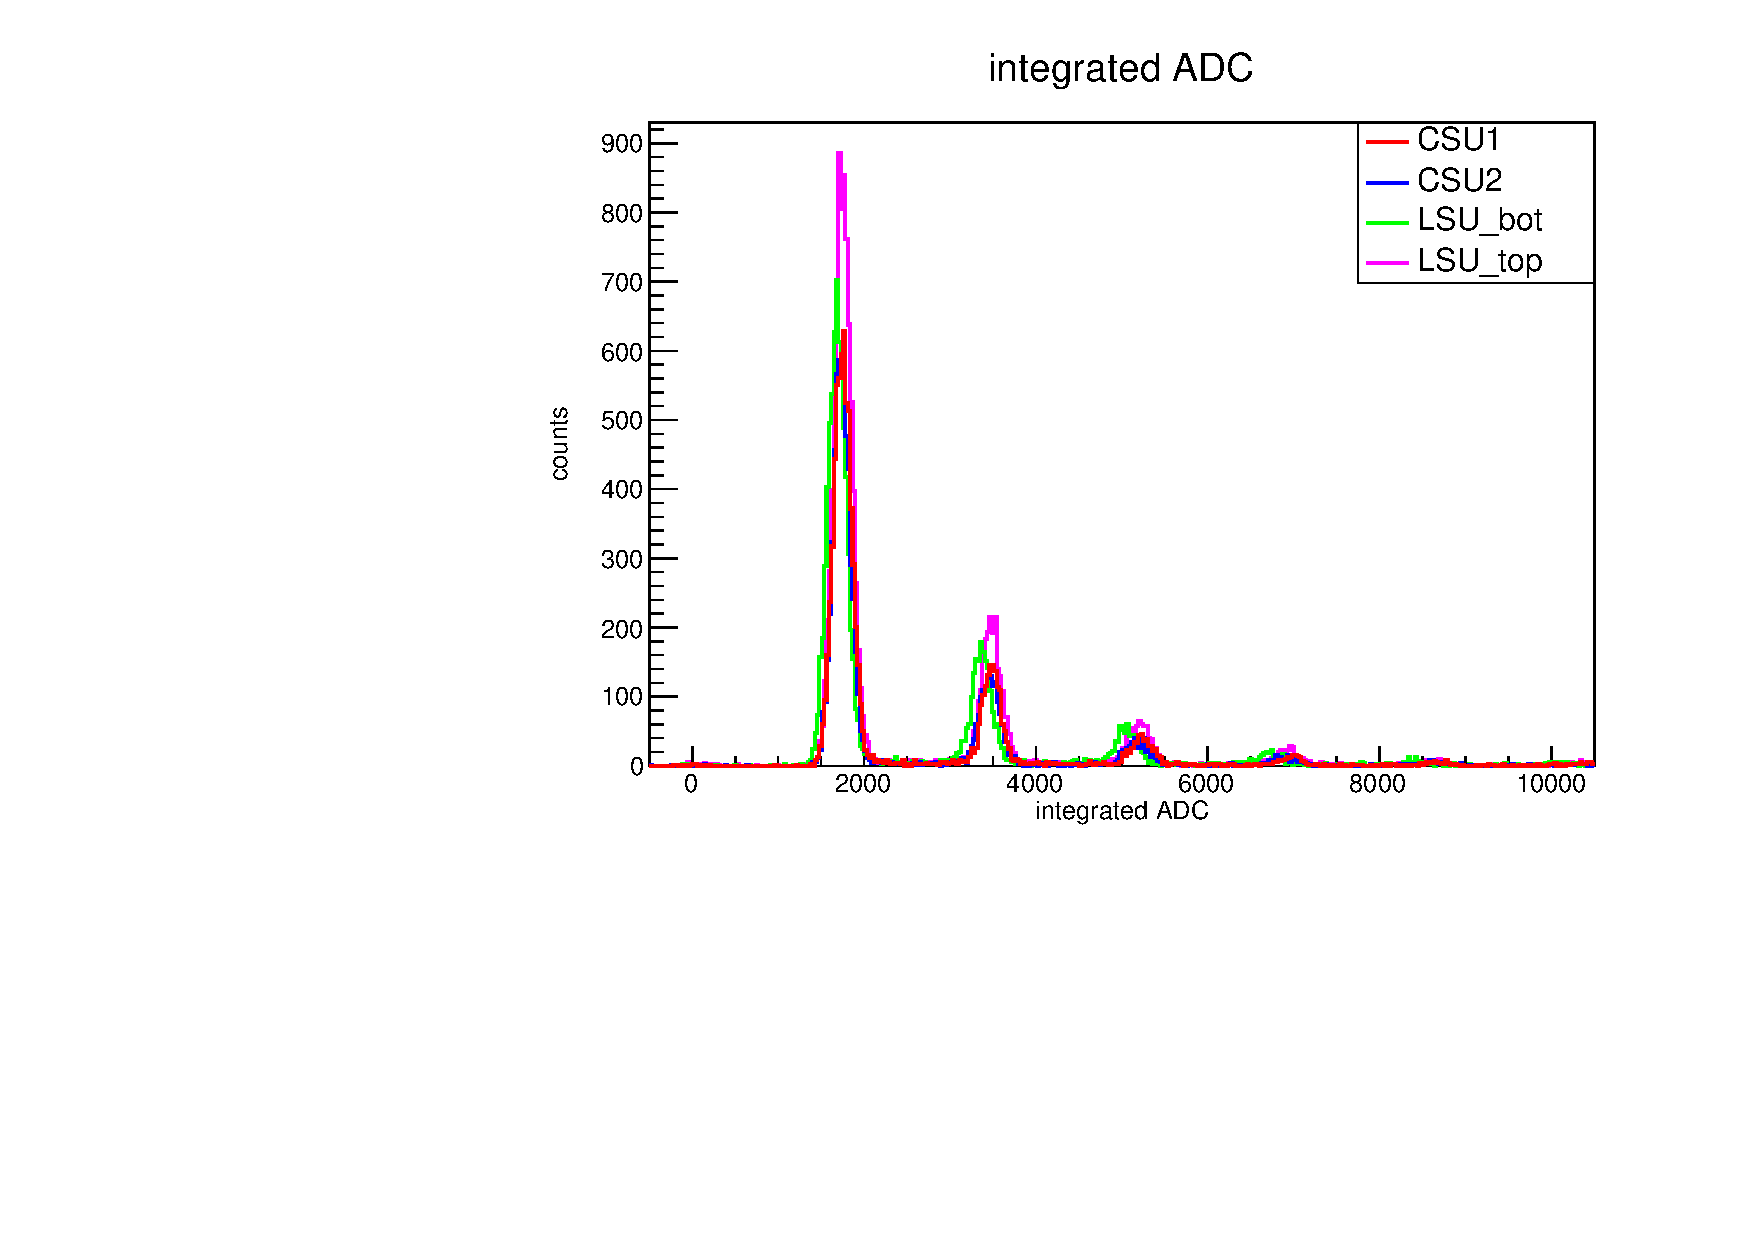
\includegraphics[angle=270,origin=c,width=.7\textwidth]{figures/integratedADC.pdf}
  \caption{Integrated ADC for the four SiPM channels.}
  \label{fig:cddfadc}
\end{figure}

\begin{figure}
  \centering
  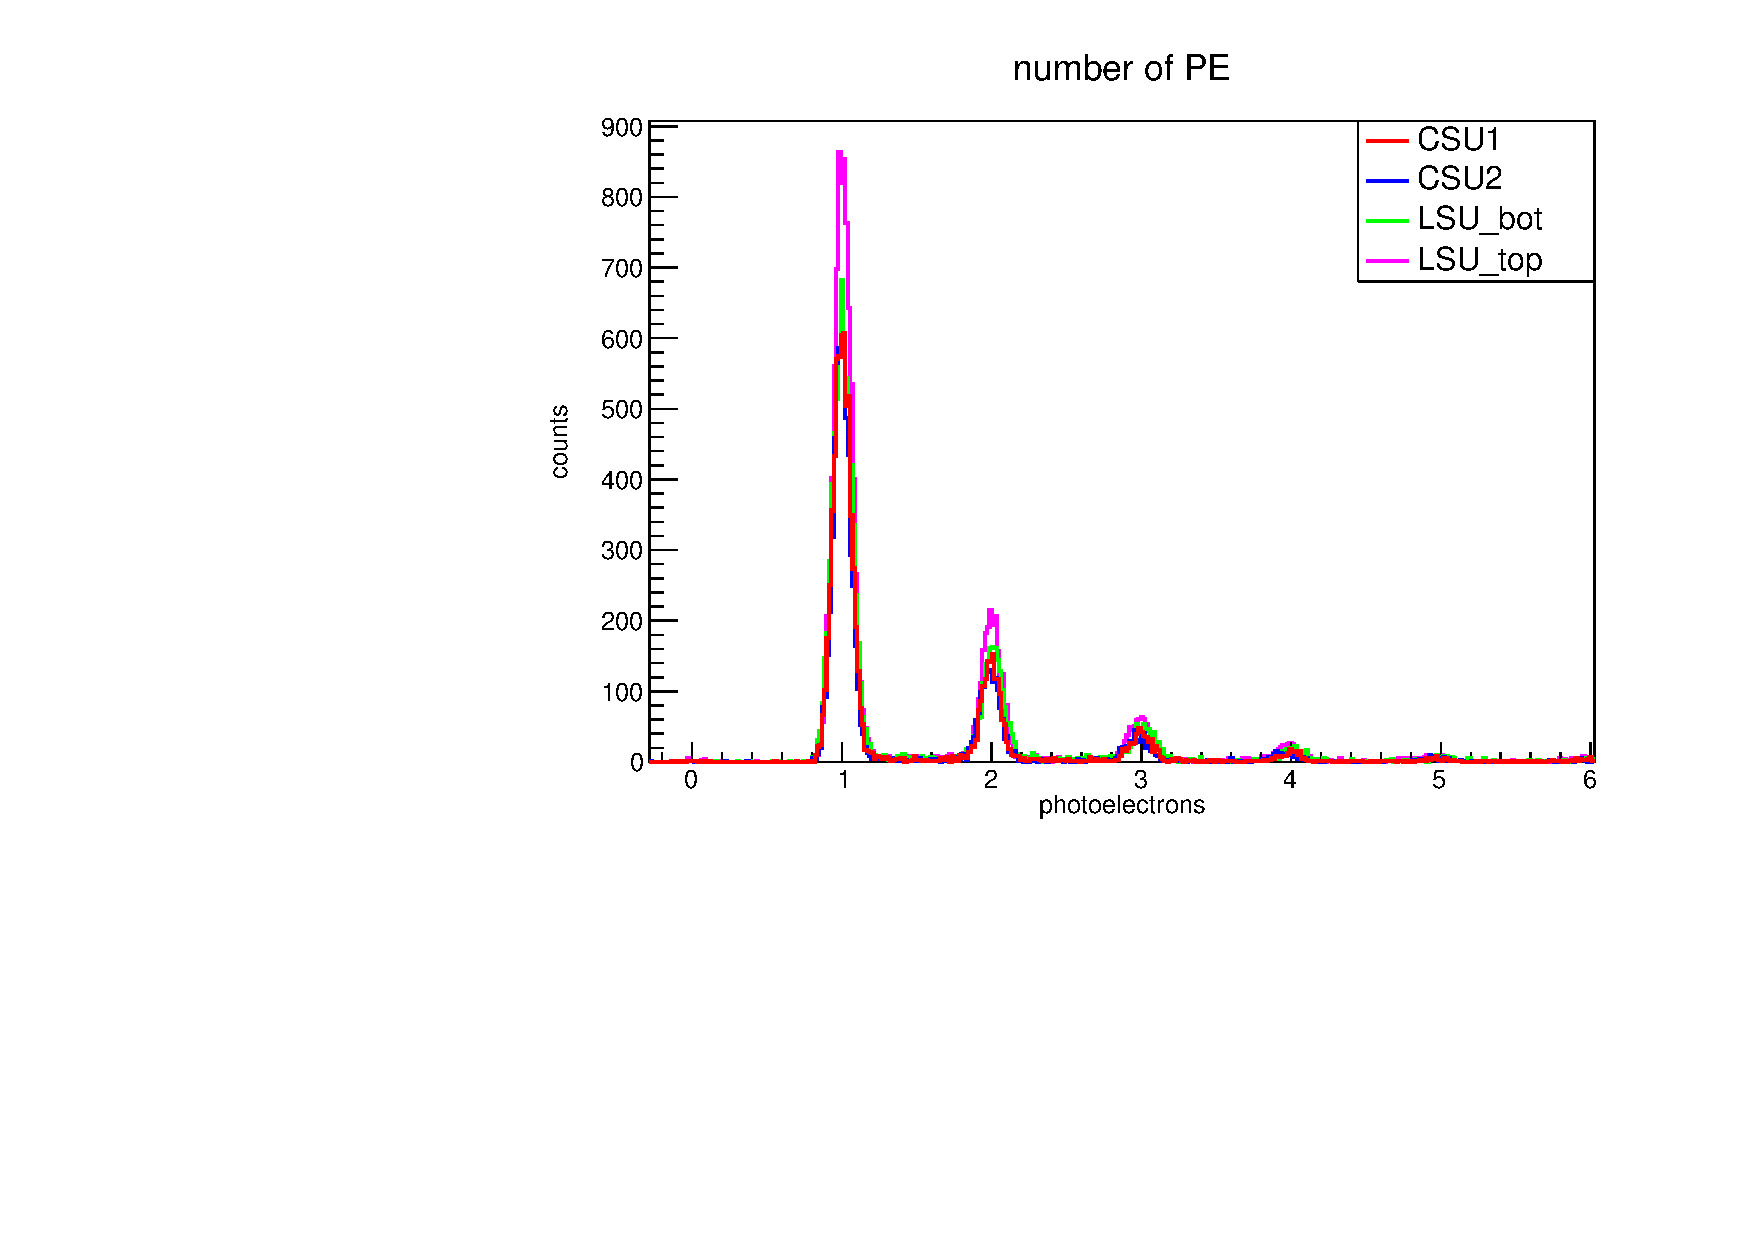
\includegraphics[angle=270,origin=c,width=.7\textwidth]{figures/calibrated_spectra.pdf}
  \caption{ADC to photoelectron calibration for the four SiPM channels.}
  \label{fig:cddfcalibrated}
\end{figure}

Figure~\ref{fig:cddfcalibrated} shows calibrated photoelectron(PE) spectra for the four channels. The calibration was done by assigning the first peak to 1 PE, the second to 2 PE, etc.

\section[NOvA]{NO$\nu$A}

%\section*{References}
%\begin{thebibliography}{10}
%\bibitem{ref1} J.~Doe, Article name, \textit{Phys. Rev. Lett.}
%
%\bibitem{ref2} J.~Doe, J. Smith, Other article name, \textit{Phys. Rev. Lett.}
%
%\bibitem{web} \href{http://www.google.pl}{www.google.pl}
%\end{thebibliography}

\end{document}

